% ============================================================
\section{Experiments}
\label{sec:experiments}
Numerical experiments are conducted to validate the proposed PIHS algorithm.
The algorithms are implemented in \texttt{Python3} and \texttt{PyBullet}~\cite{coumans2019}
on a computer with an Intel Core i9-14900KF and an NVIDIA RTX 4080.
Videos are provided as multimedia attachments.
\subsection{Numerical Simulations}
\label{subsec:sim}
% ========================================


\subsubsection{Setup and Configuration}\label{subsec:sim-setup}

The simulation uses a step size of $\Delta t=1/240$\,s and a control
period of $1/40$\,s. Robots are modeled as disk or box pushers consistent
with the $W$-clearance definition, while movable obstacles have masses
uniformly sampled from $[5,15]$\,kg. A trial succeeds when the external vehicle
reaches its goal through a $W$-clear path.
The nominal scenario uses an $8\times5$\,m workspace with bottleneck-forming
bar obstacles and randomly distributed movable objects. Two robots clear
$10$--$15$ movable obstacles under minimum-separation constraints. Unless
otherwise stated, comparisons and ablations are conducted on Scenario~1 with
$10$ movable obstacles over $40$ trials, while Scenario~2 with
$14$ obstacles provides an additional cluttered case. All methods use the same
robot footprints, obstacle configurations, collision/reachability checks, and
execution simulator, and are given the same per-trial timeout of $800$\,s and
planning budget of $20{,}000$ control steps; unsuccessful trials are assigned
the $800$\,s cap in the planning-time statistics.

%==============================
\subsubsection{Results}


Two representative simulation runs are shown in Fig.~\ref{fig:main_result}.
In Scenario~1 ($10$ movable obstacles, two robots) the start and goal belong to
different $W$-clearance faces, so the planner clears the blocked passage with
$6$ pushes in $7.4$\,s and the execution finishes in $42.27$\,s with the
start face containing the goal. Scenario~2 ($14$ obstacles) requires a $9$-push
plan in $11.2$\,s and $61.27$\,s of execution. In both cases the executed
pushes progressively enlarge the reachable $W$-clearance region until a
complete $W$--clear path is found, as shown by the expanding blue start face in
the WCCG overlays.



% ========================================
\change{
\subsubsection{WCCG Connectivity Validation}
\label{subsec:wccg-validation}

WCCG is compared against continuous C-space (CC) and a rasterized reference at
$0.02$\,m (FR) on $300$ random scenarios (Table~\ref{tab:wccg-validation}):
CC and FR agree in $296$ cases, WCCG agrees with CC in all $300$ with zero
FP/FN, and a query costs $1.07$\,ms against $1.36$\,ms (CC) and $243$\,ms (FR),
while additionally supplying the gap graph needed by PIHS.
}

\begin{table}[t]
\centering
\caption{\change{WCCG connectivity validation and mean runtime.}}
\label{tab:wccg-validation}
\vspace{-2mm}
\scriptsize
\setlength{\tabcolsep}{3.2pt}
\renewcommand{\arraystretch}{1.0}
\begin{tabular}{lccccc}
\hline
& & & \multicolumn{3}{c}{Time (ms)}\\
Type & CC=FR & FP/FN$^\dagger$ & CC & FR & WCCG\\
\hline
Convex     & 100/100 & 0/0 & 1.23 & 282.9 & \textbf{0.86}\\
Non-convex & 98/100  & 0/0 & 1.51 & 204.1 & \textbf{1.30}\\
Mixed      & 98/100  & 0/0 & 1.33 & 242.4 & \textbf{1.05}\\
\hline
Total      & 296/300 & \textbf{0/0}
           & 1.36 & 243.1 & \textbf{1.07}\\
\hline
\end{tabular}

\vspace{0.5mm}
{\scriptsize $^\dagger$WCCG errors on CC--FR-consistent cases. All runtimes are
measured in one harness over the same $300$ scenes, with WCCG served by its
compiled backend;}
\vspace{-5mm}
\end{table}
% ========================================
\begin{table}[t]
  \centering
  \begin{threeparttable}
  \caption{Performance comparison and ablations on Scenario~1 over $40$ randomized trials.}
  \label{tab:main_ablation}
  \setlength{\tabcolsep}{2.7pt}
  \renewcommand{\arraystretch}{0.95}
  \begin{tabular}{lccccc}
  \toprule
  Method / Variant & Succ.(\%) & PT (s) & ET (s) & \#Sims & \#Pushes \\
  \midrule
  DFS-WCCG            & 25.0  & $>$100.0 & 51.2 & $>$500 & 8.0 \\
  SL-Push (offline)   & 62.5  & 0.06     & 44.1 & 0.0    & 7.3 \\
  SL-Push (sim)       & 75.0  & 18.2     & 64.6 & 20.0   & 10.2 \\
  Rec-NAMO            & 37.5  & 13.3     & 42.4 & 0.0    & 7.8 \\
  \textbf{PushAround (ours)}
                       & \textbf{97.5} & \textbf{10.3} & \textbf{28.6}
                       & \textbf{121.5} & \textbf{6.0} \\
  \midrule
  w/o gap-lookahead    & 82.5 & 16.9 & 35.2 & 178.3 & 7.2 \\
  w/o mode-cache       & 92.5 & 17.1 & 33.4 & 164.6 & 6.5 \\
  w/o quick-pass       & 90.0 & 23.6 & 41.9 & 208.2 & 6.1 \\
  w/o reinsertion      & 85.0 & 12.8 & 31.1 & 151.7 & 7.8 \\
  \bottomrule
  \end{tabular}
  \end{threeparttable}
\end{table}
% ========================================

% ========================================
\begin{figure}[t!]
  \centering
  \vspace{-0.1in}
  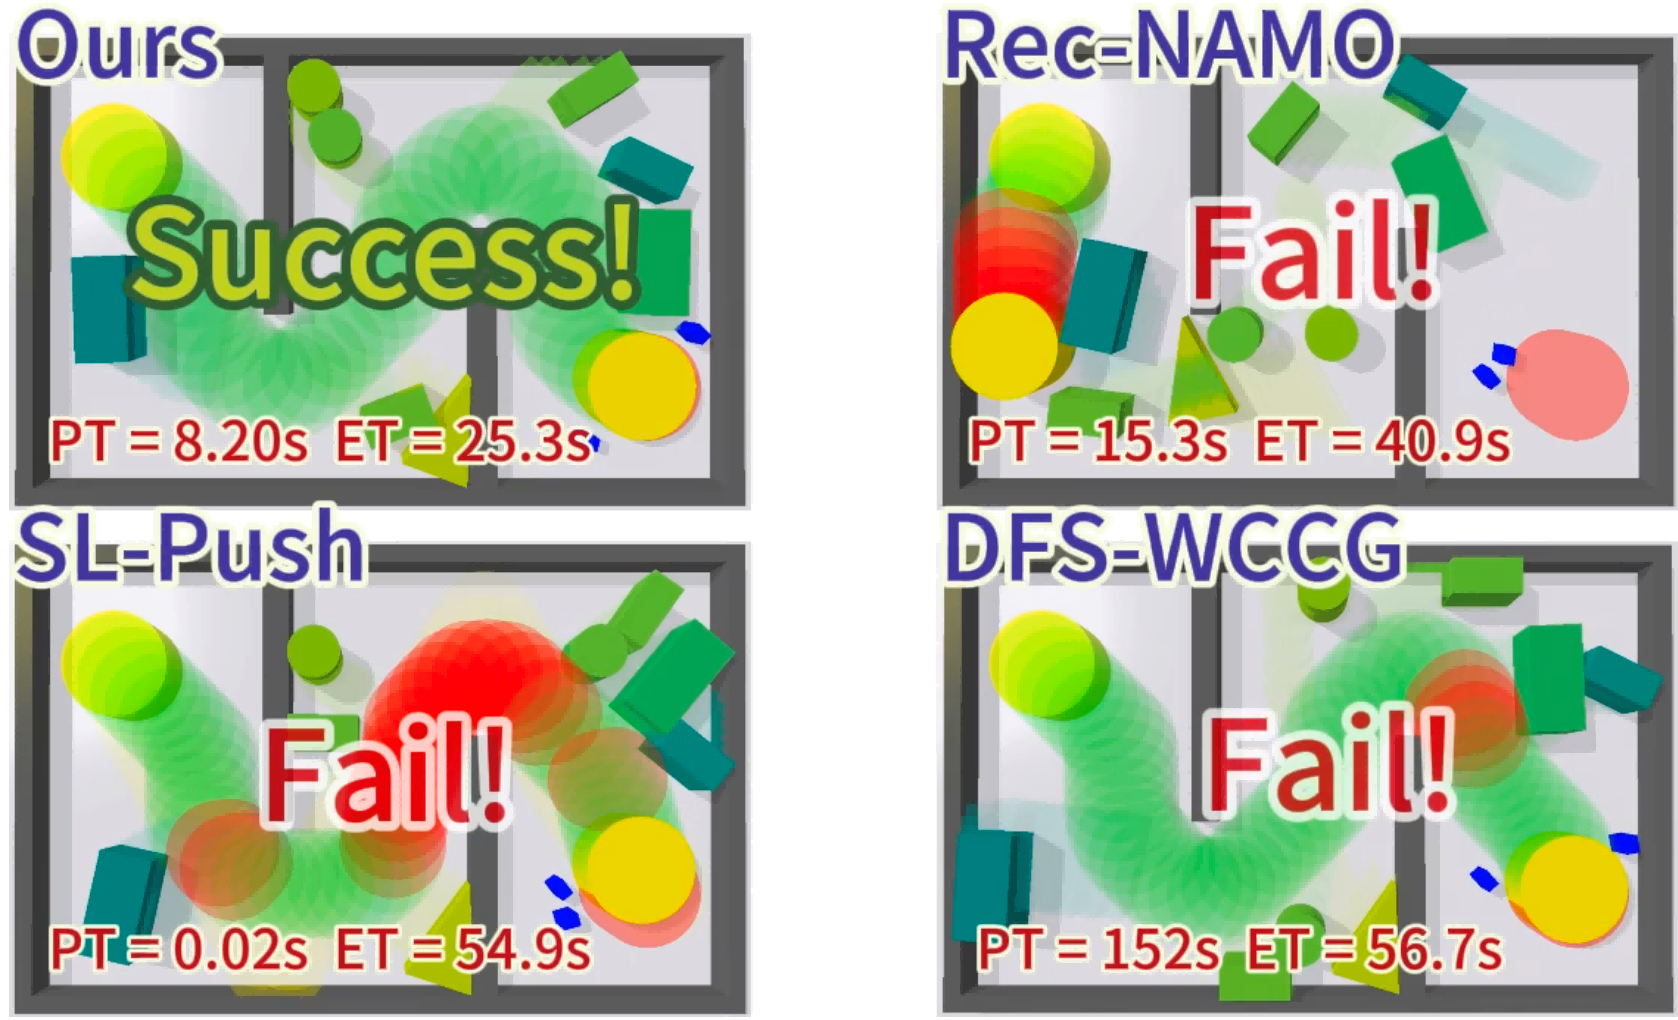
\includegraphics[width=0.8\columnwidth]{figures/compare.png}
  \vspace{-0.1in}
  \caption{Failure cases by baselines Rec-NAMO, SL-Push and DFS-WCCG.}
  \label{fig:baseline}
  \vspace{-0.2in}
\end{figure}
% ========================================

\subsubsection{Comparisons}\label{subsec:comparisons}
Four baselines are evaluated on Scenario~1 over $40$ randomized trials under
the same $W$-clearance criterion, object distribution, and simulator:
\textbf{DFS-WCCG} (WCCG-guided search with fixed pushes), \textbf{SL-Push}
(offline and simulation-validated variants), and \textbf{Rec-NAMO} (recursive
NAMO)~\cite{stilman2007manipulation,yao2024local,saxena2023planning,ren2025search}.
Table~\ref{tab:main_ablation} shows that PushAround reaches the highest success
rate ($97.5\%$) and the lowest combined planning-and-execution time ($38.9$\,s).
DFS-WCCG needs more than $100$\,s of planning (exponential branching); SL-Push
(offline) plans in $0.06$\,s but many displacements fail in execution
($62.5\%$); SL-Push (sim) reaches $75.0\%$ at $18.2$\,s planning and $10.2$
pushes; Rec-NAMO often fails to build a connected $W$--clear corridor in dense
clutter. Figure~\ref{fig:baseline} shows representative baseline failures.


% Four baselines are evaluated on Scenario~1 over $40$ randomized trials
% under the same W--clearance criterion, object distribution, and
% simulator: \textbf{DFS-WCCG}, a WCCG-guided depth-first search with
% fixed axis-aligned pushes; \textbf{SL-Push (offline)}, which clears
% route blockers without physics validation; \textbf{SL-Push (sim)},
% which validates the same route in simulation; and \textbf{Rec-NAMO},
% which combines Dijkstra routing with local push decomposition. As shown
% in Table~\ref{tab:main_ablation}, PushAround achieves the highest
% success rate of $97.5\%$ and the lowest combined planning and execution
% time of $38.9$\,s. DFS-WCCG suffers from exponential branching,
% SL-Push (offline) often produces unrealizable displacements,
% SL-Push (sim) improves feasibility at the cost of longer planning and
% more pushes, and Rec-NAMO often fails to complete a connected
% W--clear corridor in dense clutter.

%==============================
\subsubsection{Ablation Studies}
Four internal ablations are conducted: \textbf{w/o gap-lookahead} (frontier
gaps ranked without downstream costs), \textbf{w/o mode-cache} (no warm start
from previously validated modes), \textbf{w/o quick-pass} (all candidates
evaluated by rollout), and \textbf{w/o reinsertion} (temporarily failed nodes
not reconsidered). Table~\ref{tab:main_ablation} shows that gap-lookahead and reinsertion mainly
improve robustness (success drops by more than $10\%$ when either is removed),
whereas mode-cache is a warm start and only lowers success to $92.5\%$.
Quick-pass affects efficiency: without it simulations rise from $121.5$ to
$208.2$ and planning from $10.3$ to $23.6$\,s.

\change{

\subsubsection{Scalability and Robustness Analysis}
\label{subsec:generalization}

Generalization is further evaluated in the same $8\times8$\,m workspace by
scaling the obstacle density~$M$, the robot-team size~$N$, and the
execution-side physics parameters;
Table~\ref{tab:generalization} summarizes representative settings and
Fig.~\ref{fig:density_scaling} plots the complete density sweep.
\textbf{(1) Obstacle density:} with two robots and $10$ trials per density,
PushAround keeps a $100\%$ success rate for all $M\in[15,45]$ while its mean
planning time grows from $2.5$ to $53.4$\,s, whereas all baselines solve none of
the $M{=}45$ trials and removing recursive pushes lowers success to $70\%$
(Fig.~\ref{fig:scalability_scenes} shows representative runs).
\textbf{(2) Robot-team size:} at $M{=}30$, PushAround solves all ten trials at
$N{=}2$, $3$, and $4$, after two mode-generation refinements: bounded
backtracking contact assignment removes the robot-order sensitivity of greedy
replacement, and when no full-team assignment exists for a task, one robot is
released for that single push and re-activated afterwards, with a penalty
favoring full-team modes. Since the fallback belongs to the shared mode
generator, the baselines benefit as well
(Table~\ref{tab:generalization}); PushAround is nevertheless the only method
that solves all ten trials at every team size and the most economical, e.g., at
$N{=}4$ with $29.2$\,s of planning, $110.1$\,s of execution and $10$ pushes
versus $101.9$\,s, $175.9$\,s and $14$ for DFS-WCCG, and $171.7$\,s of
execution and $20$ pushes for SL-Push (sim).
\textbf{(3) Physics mismatch:} with planning on the nominal model and only
the execution simulator perturbed (one parameter at a time), PushAround
succeeds in $156$ of $160$ perturbed trials ($97.5\%$; nominal $10/10$),
the four failures being one low-friction planning failure and three budget
timeouts. Under the same $\pm40\%$ perturbations the baselines are far less
robust: SL-Push (sim) averages $32.5\%$ success ($0\%$ under the strongest
friction and force reductions) and DFS-WCCG $57.5\%$ at an order of magnitude
higher planning time.

}
\begin{table}[t]
\caption{\change{Scalability and robustness under obstacle density,
robot-team size, and execution-side physics mismatch.}}
\label{tab:generalization}
\centering
\footnotesize
\renewcommand{\arraystretch}{1.15}
\setlength{\tabcolsep}{3pt}
\begin{tabular}{l c c c c}
\hline
Case & Trials & Succ.(\%) & $PT$ (s) & $ET$ (s)\\
\hline
\multicolumn{5}{l}{\emph{Obstacle density} (PushAround, $N{=}2$, nominal)}\\
$M=15$ & 10 & 100  & $2.5\pm0.9$    & $37.1\pm21.0$\\
$M=30$ & 10 & 100  & $11.7\pm3.7$   & $100.9\pm34.7$\\
$M=45$ & 10 & 100  & $53.4\pm24.5$  & $272.7\pm97.4$\\
\hline
\multicolumn{5}{l}{\emph{Robot-team size} ($M{=}30$, nominal; $10$ trials per cell)}\\
PushAround, $N{=}3$ & 10 & 100 & $30.0\pm12.7$ & $97.3\pm42.1$\\
PushAround, $N{=}4$ & 10 & 100 & $29.2\pm8.9$  & $110.1\pm33.1$\\
SL-Push, $N{=}3$ & 10 & 80 & $30.0\pm46.3$ & $193.3\pm111.3$\\
SL-Push, $N{=}4$ & 10 & 80 & $23.4\pm18.2$ & $171.7\pm61.2$\\
DFS-WCCG, $N{=}3$ & 10 & 100 & $142.6\pm183.1$ & $178.1\pm72.1$\\
DFS-WCCG, $N{=}4$ & 10 & 90 & $101.9\pm103.9$ & $175.9\pm113.6$\\
\hline
\multicolumn{5}{l}{\emph{Physics mismatch} ($M{=}30$, $N{=}2$)}\\
Nominal            & 10  & 100  & $16.8\pm3.4$  & $104.7\pm37.4$\\
Mass $\times0.6$--$1.4$          & 40  & 100  & $16.8\pm5.4$  & $105.9\pm44.6$\\
Lateral fric. $\times0.6$--$1.4$ & 40  & 97.5 & $16.5\pm5.7$  & $114.0\pm48.5$\\
Spin fric. $\times0.6$--$1.4$    & 40  & 97.5 & $15.2\pm3.6$  & $100.1\pm35.7$\\
Force limit $\times0.6$--$1.4$   & 40  & 95.0 & $18.9\pm10.9$ & $115.9\pm58.5$\\
All perturbed      & 160 & 97.5 & $16.9\pm7.0$  & $108.9\pm47.4$\\
\hline
\end{tabular}

\vspace{-1mm}
\begin{flushleft}
\footnotesize
Each perturbed physics row scales one execution-side parameter over the
factor range shown while the others remain nominal.
\end{flushleft}
\vspace{-4mm}
\end{table}
% ========================================
\begin{figure}[t!]
  \centering
  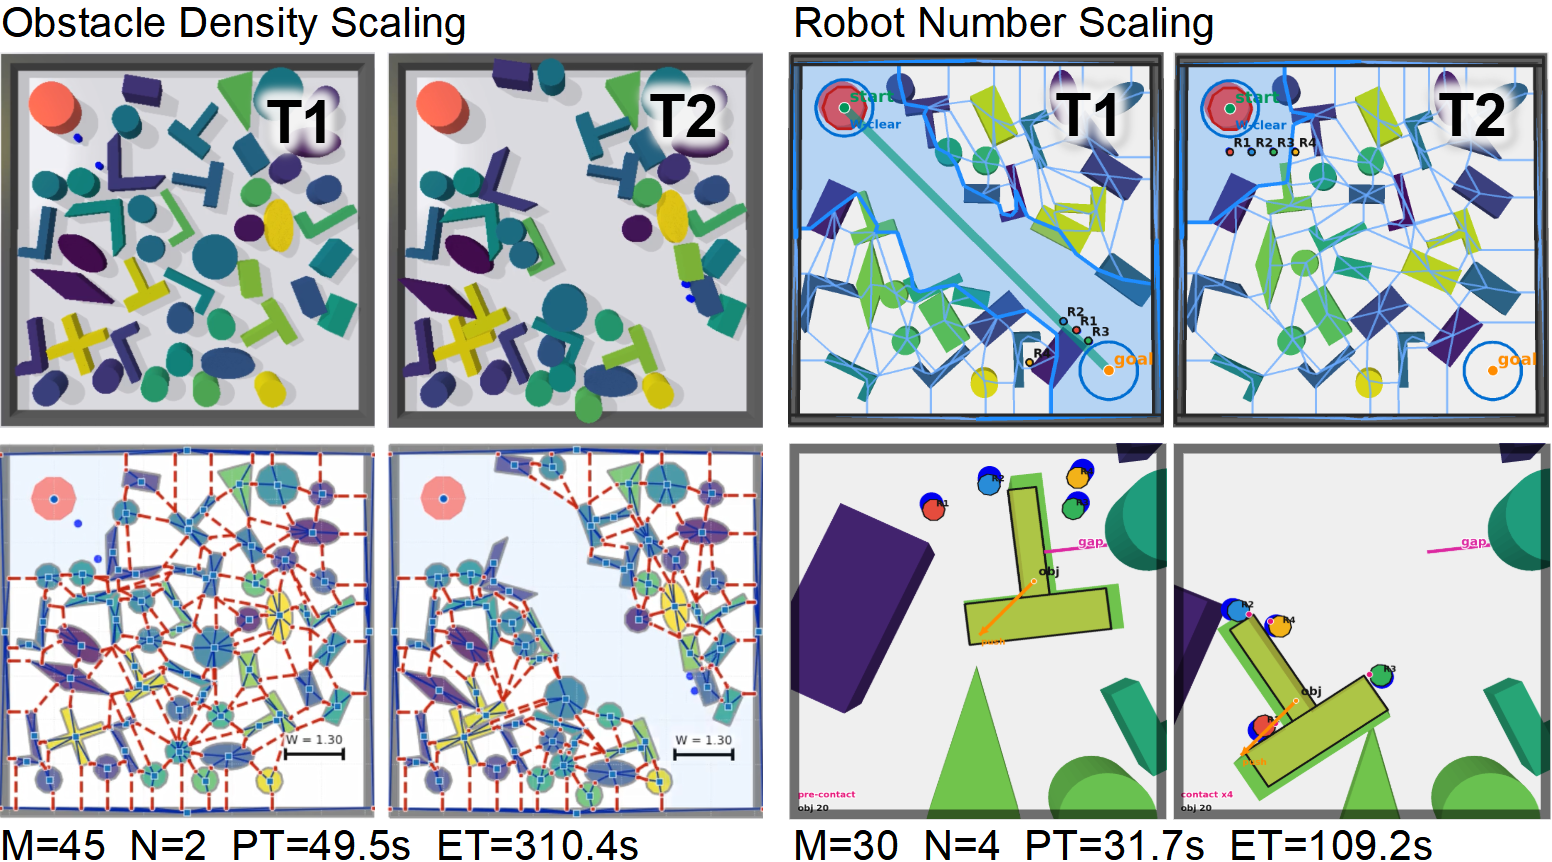
\includegraphics[width=0.8\columnwidth]{figures/obs_rob_scale.png}
  \vspace{-0.09in}
  \caption{
  Scalability of the clearing process.
  \textbf{Left:} obstacle-density scaling with $M{=}45$ movable objects and two
  robots, showing snapshots during the clearing (\textbf{top}) and the
  corresponding WCCG overlays with the start face in blue (\textbf{bottom}).
  \textbf{Right:} robot-team scaling with $M{=}30$ objects and four robots,
  showing the global initial and final states (\textbf{top}) and magnified views
  of one pushing task before contact and during the push (\textbf{bottom}).
  }
  \label{fig:scalability_scenes}
  \vspace{-0.1in}
\end{figure}
% ========================================
% ========================================
\begin{figure}[t!]
  \centering
  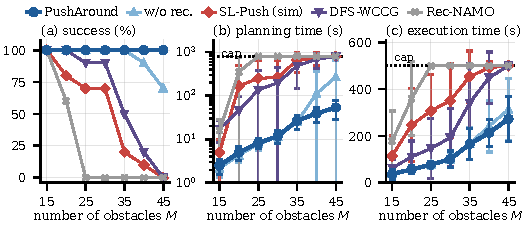
\includegraphics[width=0.95\columnwidth]{figures/density_comparison.pdf}
  \vspace{-0.15in}
  \caption{
  Obstacle-density scaling ($8\times 8$\,m, $10$ independent seeds per density).
  \textbf{(a)} Success rate; \textbf{(b)} mean planning time, with unsuccessful
  trials capped at the $800$\,s budget (dotted line); \textbf{(c)} mean execution
  time of the successful trials (Rec-NAMO has none beyond $M{=}20$). Error bars
  denote one standard deviation; PushAround keeps a $100\%$ success rate over the
  whole range, whereas the baselines degrade sharply.
  }
  \label{fig:density_scaling}
  \vspace{-3mm}
\end{figure}
% ========================================
% ========================================
\begin{figure*}[t!]
  \centering
  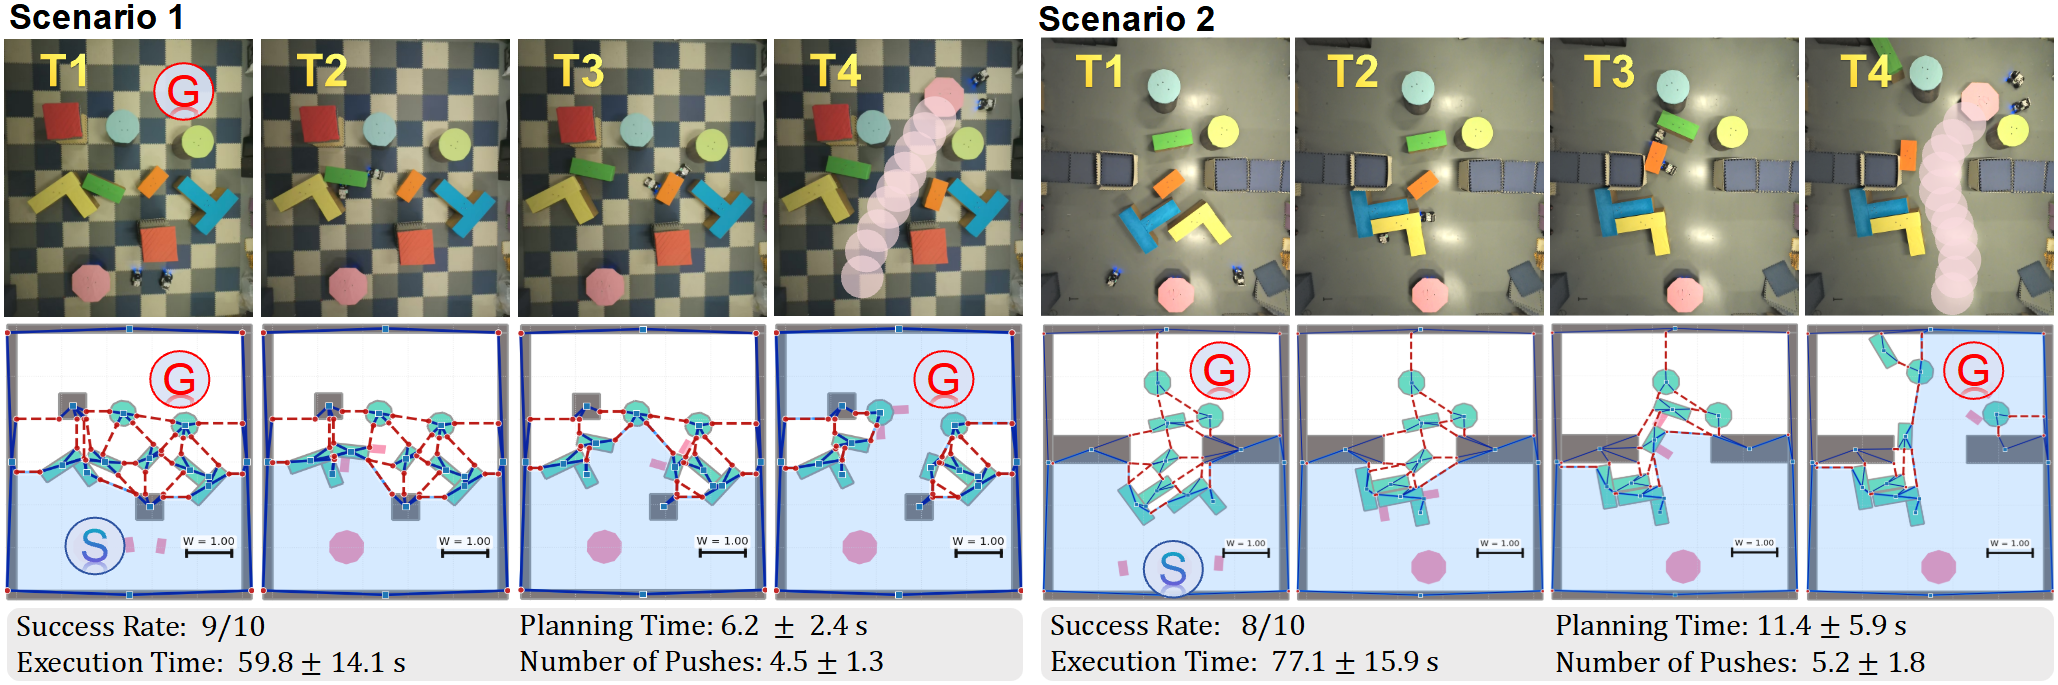
\includegraphics[width=0.8\linewidth]{figures/hardware.png}
  \vspace{-4mm}
  \caption{Real-world pushing experiments with the execution--planning alignment(over~$20$ runs and $2$ scenarios).
    \textbf{Top:} snapshots of two robots pushing obstacles in a \(5{\times}6\,\mathrm{m}\) workspace
    with movable objects and fixed boundaries. \textbf{Bottom:} WCCG overlays with the start face in blue. 
  }
  \vspace{-4mm}
  \label{fig:hardware}
\end{figure*}
% ========================================
\subsection{Hardware Experiments}\label{subsec:hardware}

\subsubsection{System Description}\label{subsec:exp-description}
Experiments use a $5\times6$\,m workspace of interlocking $0.6\times0.6$\,m
foam mats (Fig.~\ref{fig:hardware}), $2$ UGVs and $6$ cardboard-box movable
obstacles. Robots and movables each carry three to four motion-capture markers
whose global poses are streamed to \texttt{PyBullet} in real time.
\change{
The two Mecanum UGVs are controlled through planar velocity commands, while
the optimized contact forces are used only for feasibility evaluation rather
than direct motor control. Motion capture provides the current robot and
object poses, which are compared with the successor state predicted by
$\mathsf{EvalSim}$: a push is deemed to deviate and triggers replanning only
when the measured object position error exceeds $0.3$\,m or its orientation
error exceeds $\pi/4$. The threshold is deliberately loose, tolerating a
slight over-push or off-axis push.}
Movables are randomly placed for each trial.

\subsubsection{Results}\label{subsec:exp-results}
Two representative real-world runs are shown in Fig.~\ref{fig:hardware}.
In Scenario~1, PIHS breaks five candidate gaps within $6.5$\,s using $12$ node
expansions, $49$ visited snapshots and search depth $6$; the four-task schedule
first pushes and rotates the yellow L-shaped object to open a gap near an
immovable obstacle, then pushes the green and orange objects apart until the
green cylinder is pushed to the right and a $W$--clear path is established at
$t=52\,$s.
In Scenario~2, PushAround succeeds in $8/10$ trials with an average of $5.2$
pushes and $11.4$\,s of planning; it first selects a direct push on the blue
L-shaped object, which also moves the adjacent T-shaped block and opens the
first gap into the narrow passage.
\change{This neighboring-object motion is not a separately encoded action but
an emergent outcome of the coupled rigid-body rollout in $\mathsf{EvalSim}$,
whose snapshot is used to update the WCCG and continue replanning.}
The complete execution takes $77.1$\,s on average with $15.9$\,s deviations,
mainly from direction-dependent force limits, drifting, and Mecanum-wheel
slippage near $45^\circ$ motion directions, which are compensated by online
replanning.
